\chapter{Design}

\section{Architecture Overview}

The Connectivity Manager is logically located between the EMM and the cloud infrastructure and provides the following two functionalities:
\begin{itemize}
\item \textbf{Optimal Instance Placement:} During the deployment of a stack an algorithm chooses where individual instances are placed within the cloud infrastructure.
\item \textbf{Service-Level Agreement Enforcement:} Depending on the services that an instance provides to the rest of the stack, certain requirements for its network performance need to be fulfilled.
\end{itemize}

\begin{figure}[H]
\centering


\includegraphics[width=0.5\textwidth]{images/design/functional_architecture}

\caption{High-level architecture of the Connectivity Manager}
\end{figure}

The \textit{Instance Placement Engine} determines if and where the instances should be deployed. It does so by comparing the current utilization and capacity of the available compute nodes within the availability zone.

The \textit{QoS Manager} enforces different QoS policies based on the type of service that the instance is grouped in. A guaranteed and maximum bit-rate for the network port of an instance can be set. This way a certain network performance can be insured opposed to the commonplace best-effort packet delivery.

\section{Interface between CM Manager \& Agent}

The Connectivity Manager and Agent are two separate applications that communicate using a ReST API. 

\begin{figure}[H]
\centering

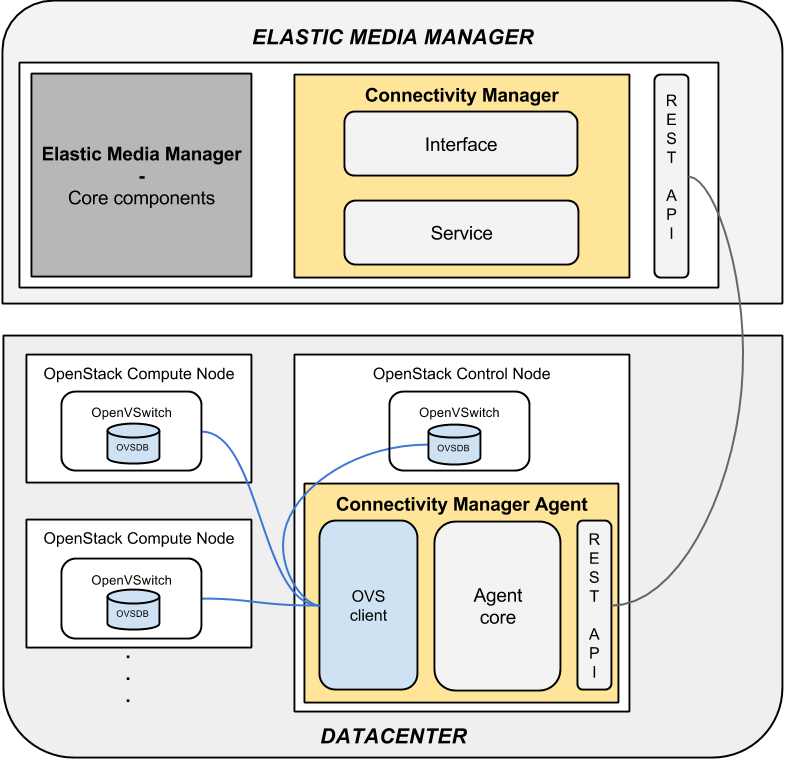
\includegraphics[width=0.6\textwidth]{images/design/modular_architecture_cm_cma}

\caption{Minimized architecture of the Connectivity Manager and its integrations}
\end{figure}

This design was chosen first of all because the Connectivity Manager is integrated within the EMM, which is required to be placed outside of the data center. Second of all the Connectivity Manager Agent needs access to the OVSDB on the compute nodes and consequently needs to be within the internal management network of the OpenStack infrastructure.

The sequence diagram below displays the work-flow that the CM passes during the run-time.

\begin{figure}[H]
\centering

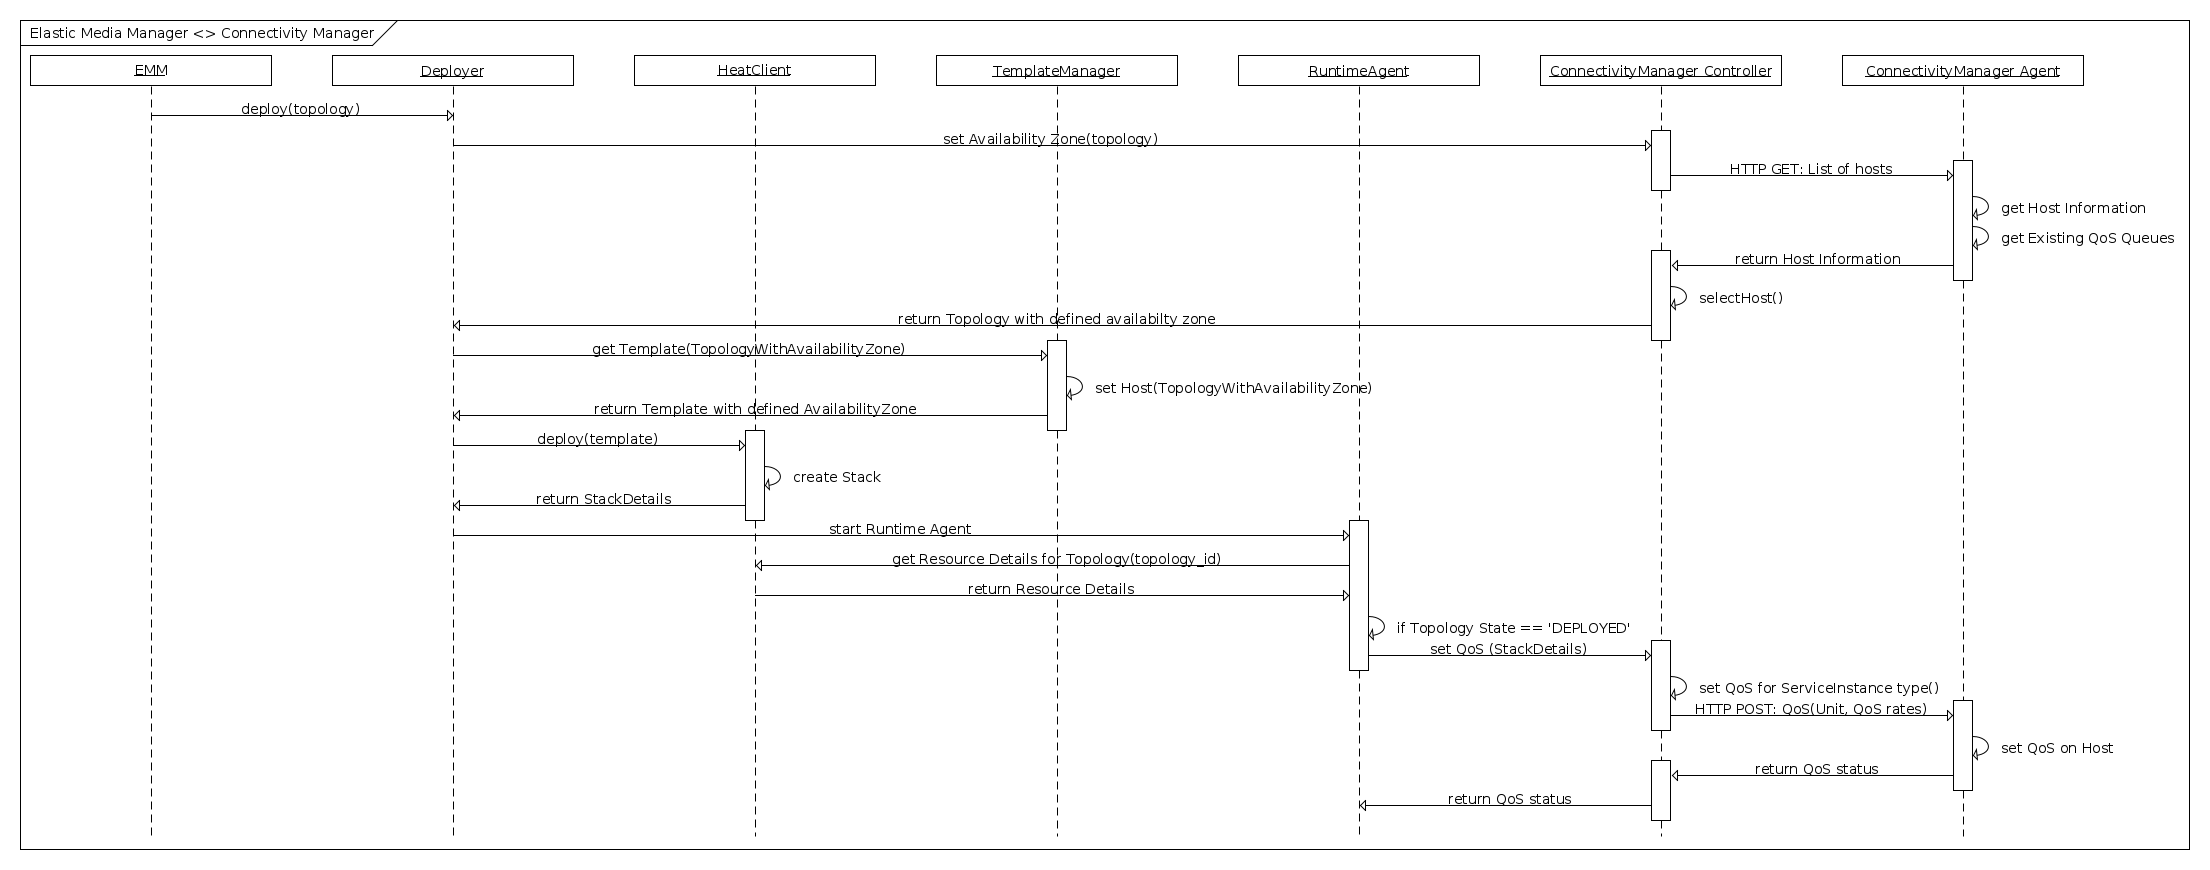
\includegraphics[width=0.9\textwidth]{images/design/sequence_diagram}

\caption{Deployment of stack \& Assignment of QoS policies}
\end{figure}

As visible in the above figure, the Connectivity Manager receives the Topology object that contains a description of the configuration and specifications of the whole stack. For the placement decision the CM to needs to get the information about the current state of the infrastructure. This exchange with the CM Agent occurs through the HTTP API. Upon reception of that data, the placement algorithm sets the availability zone for each instance within the topology. The topology is then converted into a Heat template by the Template Manager. Once the template got deployed by the Heat Client the runtime agent starts. The purpose of the runtime agent is to continuously check the state of the stack. Once the stack has reached the 'DEPLOYED' state, the runtime agent requests the CM to set the QoS policies according to previously configured values. This configuration is subsequently transmitted to the CM Agent whose task is to then enable the policies on the according ports of the instances within the Open vSwitches.


\section{Design of Connectivity Manager}

The design of the Connectivity Manager is based on the framework that already exists in the Elastic Media Manager.

It consists of a highly dynamic factory, abstract interfaces and the actual implementation as a service.
The Factory Agent reads a configuration file in which the class name of the service for the according interface is defined. It then instantiates a instance from that given class. This means it is easy to replace the actual implementation while the interface to the other components can remain unchanged.

\begin{figure}[H]
\centering

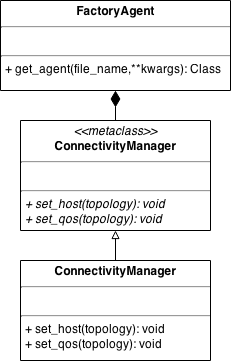
\includegraphics[width=0.2\textwidth]{images/design/cm-emm_interface_classes}

\caption{Metaclass (Interface) and implementation (Service) instantiated by Factory Agent}
\end{figure}

The Connectivity Manager interface and service only contain the methods that receive calls from the Elastic Media Manager. However additional helper classes are needed in order to provide the appropriate configuration and the communication with the Connectivity Manager Agent, as shown in the next figure.

\begin{figure}[H]
\centering

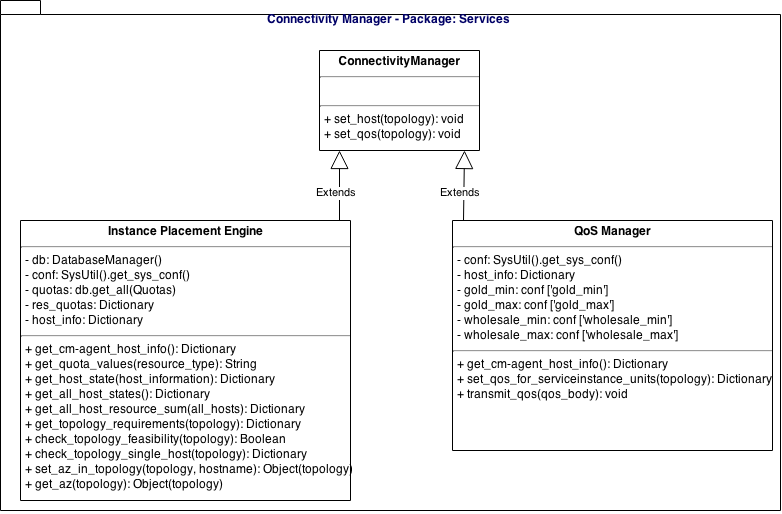
\includegraphics[width=0.6\textwidth]{images/design/cm_class_diagram}

\caption{Connectivity Manager service and its helper classes}
\end{figure}

The topology that is created by the EMM contains the following required resources for the stack:

\begin{figure}[H]
\centering

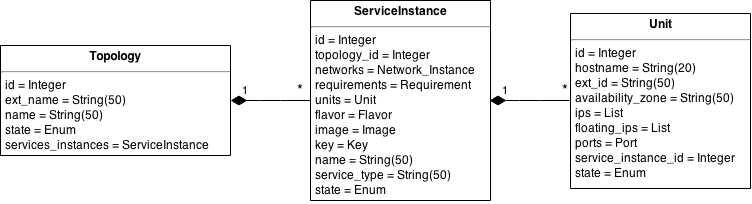
\includegraphics[width=0.8\textwidth]{images/design/cm_topology_object}

\caption{Deployment: Topology object from EMM}
\end{figure}

This object is handed over to the CM during the deployment phase. The topology can contain multiple Service Instances, which defines general parameters such as what networks the underlying instances need to be connected to, the flavor wherein the resources (e.g. amount of RAM \& CPU) are specified \cite{openstack-admin}, the image that contains the operating system and additional software packages plus the key that is needed to establish a connection to the server via SSH.

Each Service Instance can contain multiple Units (servers). Among others it contains parameters like IP addresses, the availability zone that it gets deployed on and the external ID which is unique across the whole infrastructure.



\subsection{Algorithm for Instance Placement}

The following section describes the algorithm that is used for setting the availability zone for the instances, and thus placing them in the most advantageous way based on the project requirements.

Each tenant has a set of quotas which limit the resource usage within the OpenStack infrastructure. Limitations can be made based on the following resource types (excerpt): Amount of instances, vCPU's, RAM, Floating IP addresses and fixed IP addresses \cite{openstack-admin}.

Considering the requirement to have optimal connectivity between individual instances, it is preferable to position them on the same compute node, given that its resources allow this.

\begin{figure}[H]
\centering

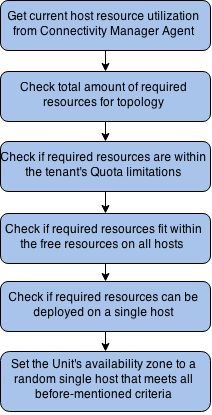
\includegraphics[width=0.25\textwidth]{images/design/cm_instance_placement_engine.png}

\caption{Instance Placement work-flow}
\end{figure}


\subsection{QoS Manager}

The QoS is deployed on the port of the internal bridge of the Open vSwitch that is connected to the virtual ethernet interface of a Unit. This design compared to deploying the same quality-of-service assurances across a whole tenant was chosen, because the traffic needs to be differentiated between the various service instances. The bandwidth rates are required to be configurable and therefore can't be hard-coded. By default the following rates and classes are set:

\begin{table}[H]
\centering

\begin{tabular}{|c|c|c|}
\hline \textbf{Name} & Minimum rate & Maximum rate \\ 
\hline Wholesale & 100 MBit/s & 1 GBit/s \\ 
\hline Gold & 100 MBit/s & 10 GBit/s \\ 
\hline 
\end{tabular} 

\caption{QoS classes and their default rates}
\end{table}


All Units that are part of the 'Media Server' service instance are associated with the Gold class and all units of other types in the topology are part of the Wholesale class.


\newpage
\section{Design of Connectivity Manager Agent}

The CM Agent is separated into the WSGI Application wherein the routes for the ReST API and the corresponding methods that will be called are defined. The Agent class calls the different Clients to get the status of the resources and make changes to their configuration.

\begin{figure}[H]
\centering

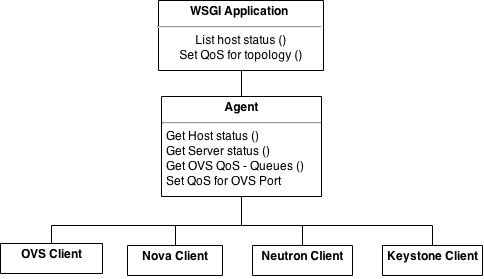
\includegraphics[width=0.8\textwidth]{images/design/cm_agent_design_class_diagram.png}

\caption{Abstract design of the Connectivity Manager Agent}
\end{figure}

For connecting to the OVSDB the OVS Client is needed on each host. It contains methods for listing all of its ports, interfaces, qos's and queues as well as for applying actions to a port, creating queues and creating new qos's.

The OpenStack Identity API is what the Keystone Client is connecting to in order to get the authentication endpoint and token for Neutron.

The Nova Client binds to the OpenStack Nova API and is required for getting the status of all Compute Nodes and the servers running on it.

Each server can have multiple network ports, which are managed by Neutron. The Neutron Client can retrieve a list of all ports for the servers that exist for a tenant.

Finally the OVS Client makes use of various calls to the OVS control tool (ovs-vsctl) for reading various tables of the OVSDB and making changes for enabling QoS on a per-port basis.

During the design process the following package structure was decided on:

\begin{figure}[H]
\centering

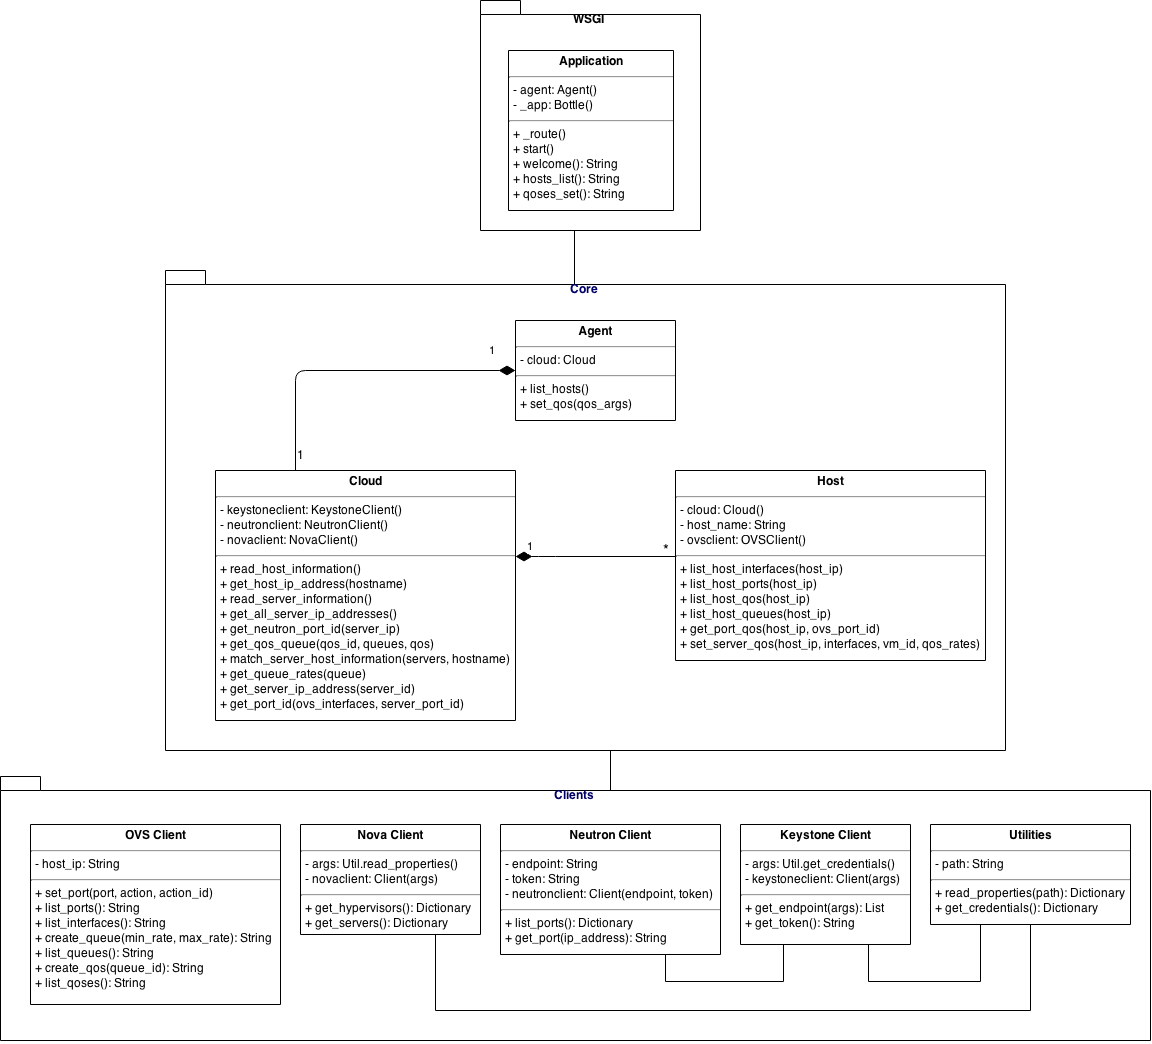
\includegraphics[width=0.8\textwidth]{images/design/cm_agent_class_diagram}

\caption{Class diagram: Connectivity Manager Agent - All packages}
\end{figure}


\subsection{API}

In the following table the ReST API that the Connectivity Manager Agent exposes to the Connectivity Manager is described:

\begin{table}[H]
\centering

\begin{tabularx}{\textwidth}{ |X|X|X|X| }
\hline HTTP method & Path & Method body & Description \\ 
\hline GET & /hosts & - & List all available hosts and their resources \\ 
\hline POST & /qoses & JSON: \{'Hostname': \{'Server ID': \{'QoS rates'\}\}\} & Set QoS rates for servers. \\ 
\hline 
\end{tabularx}

\caption{Connectivity Manager Agent - API description}
\end{table}


